\documentclass[11pt]{article}

\usepackage{graphicx}
\usepackage{url}
\usepackage{float}

\begin{document}

\begin{titlepage}
    \begin{center}
    	
\includegraphics[scale=0.10]{du.png}\par
		\begin{Huge}
			\textsc{University of Dhaka}\par
		\end{Huge}
		\begin{Large}
            Department of Computer Science and Engineering\par \vspace{0.5cm}
            CSE-3111 : Computer Networking Lab \\[12pt]	
        \end{Large}
        \textbf{Lab Report 3:}
        Implementing File transfer using Socket Programming and HTTP
GET/POST requests \\[8pt]
        \begin{large}
            \textbf{Submitted By:\\[12pt]}
            Name: Meherun Farzana\\[8pt]
            Roll No : 05\\[12pt]
            Name: Mohd. Jamal Uddin Mallick\\[8pt]
            Roll No : 07\\[12pt]
            \textbf{Submitted On : \\[12pt]}
            February 8, 2024\\[20pt]
            \textbf{Submitted To :\\[12pt]}
            Dr. Md. Abdur Razzaque\\[12pt]
            Dr. Md. Mamun Or Rashid\\[12pt]
            Dr. Muhammad Ibrahim\\[12pt]
            Redwan Ahmed Rizvee
        \end{large}
\end{center}
\end{titlepage}

\section{Introduction}
File transfer is a critical aspect of modern networking applications, facilitating the exchange of data between systems. This lab report focuses on implementing file transfer using two essential techniques: socket programming and HTTP GET/POST requests. Socket programming provides a foundational framework for establishing communication channels between client and server applications, while HTTP protocols offer standardized methods for data exchange over the web.

\subsection{Objectives}
\begin{itemize}
    \item \textbf{Socket Programming: } Develop a file transfer mechanism using socket programming to establish communication between client and server applications.
    \item \textbf{HTTP GET/POST Requests} Implement HTTP GET and POST requests to facilitate file retrieval and submission over the network.
\end{itemize}
%%%%
%%%%
\section{Theory}
\subsection{File Transfer via Socket:}
Socket programming is the foundation of network communication, facilitating the establishment of connections between client and server applications for data exchange. File transfer via sockets refers to the process of transferring a file from one system to another over
a network connection using socket programming. File transfer via sockets offers more control over the transfer process compared to higher-level
protocols like HTTP, butalso requires manual handling of error handling, data chunking, and other
aspects of the transfer.
\subsection{File Transder via HTTP}
HTTP (Hypertext Transfer Protocol) serves as the backbone of web communication, enabling clients to request resources from servers using methods such as GET and POST. HTTP is a standard protocol
for transmitting data over the web, and is widely used for web communication between a client
(e.g. a web browser) and a server (e.g. a web server).
In file transfer via HTTP, the client sends a request to the server using either an HTTP GET
or POST request. Overall, file transfer via HTTP is a simple
and convenient way to transfer files over a network, but may not be as fast or efficient as other
methods, such as socket programming.

\section{Methodology}

\subsection{Server}
The server is initialized on a specific port and it listens for incoming requests. Whenever a client requests to connect, the server accepts the connection and provides necessary services.\\
\subsubsection{File Transfer via Socket}
In case of sockets, the server lets the client choose whether they want to get the list of available files, upload or download a file. The server can handle any type of file including text, audio, image, video etc. of all formats.
\subsubsection{File Transfer via HTTP}
In case of HTTP, the server is an HTTP server, serving GET and POST requests from clients. The client receives a response from the server indicating the success or failure
of the transfer.


\subsection{Client}
\subsubsection{File Transfer via Socket}
The client side is a program requesting service from the server. It tries to connect to the server address mentioning the particular port on which the server is serving. When the server accepts the connection, it is provided with the options of service the client can avail. The client selects whether they want to see the list of available files, upload or download a file.
\subsubsection{File Transfer via HTTP}
In case of HTTP, the client can make a \emph{GET} request to the server for a specific resource and avail it. Also it can make a \emph{POST} request for uploading new files into the server.

\section{Experimental result}

Some Snapshots of the Client Side queries can be seen in the following figures:

\subsection{Task 1: File Transfer via Socket Programming}

\subsubsection{Server:}

Server creates a socket and binds it to one of its ports. And it starts listening to incoming requests. When a client connection arrives, it accepts the connection and serves accordingly.

\subsubsection{Client: }

The client requests to connect to the server in the mentioned port. After being accepted, the client is asked what request they want to make. The client sends the request using TCP protocol and waits to receive a response.

\begin{figure}[H]
    \centering
    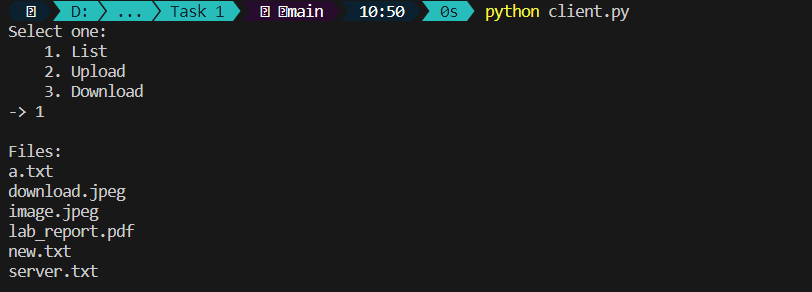
\includegraphics[scale=0.7]{Task 1/list.png} 
    \caption{Output for Option 1 (Showing all the files available in the directory)}
    \label{fig: Output for Option 1}
\end{figure}

\begin{figure}[H]
    \centering
    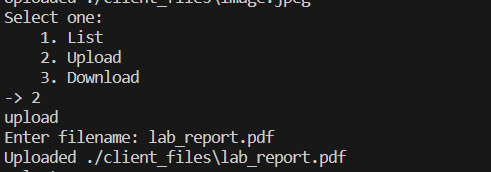
\includegraphics[scale=1.0]{Task 1/upload_pdf.png} 
    \caption{Output for Option 2 (Client uploading a pdf)}
    \label{fig: Output for Option 3}
\end{figure}

\begin{figure}[H]
    \centering
    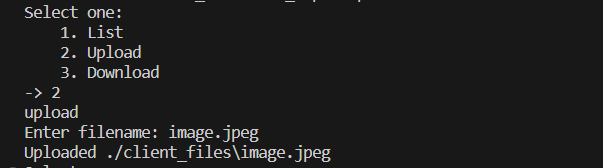
\includegraphics[scale=1.0]{Task 1/upload.png} 
    \caption{Output for Option 2 (Client uploading a jpeg file)}
    \label{fig: Output for Option 3}
\end{figure}

\begin{figure}[H]
    \centering
    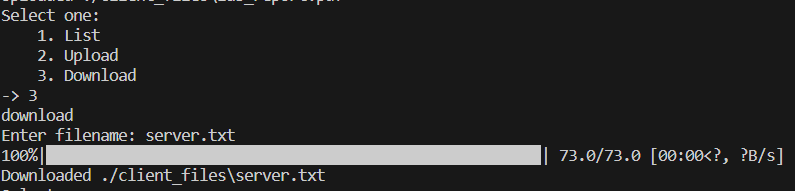
\includegraphics[scale=0.8]{Task 1/download_txt.png} 
    \caption{Output for Option 3 (Client downloading a text file)}
    \label{fig: Output for Option 3}
\end{figure}



\subsection{Task 2: File Transfer via HTTP}
\subsubsection{Server:}
HTTP file transfer server works by receiving file requests from clients, sending an HTTP response
message with the requested file, and providing the necessary information for the client to properly
display or handle the file.When a client requests a file from the server, the server sends an HTTP
response message that includes the requested file. The response message has a status code, headers,
and an optional message body that contains the file data. The headers contain information about
the file such as its size, type, and encoding.

\subsubsection{Client: }
The client side in an HTTP communication refers to the entity that initiates the request for data
from the server. The client can be a web browser, a mobile app, or any other software that needs to
retrieve data from an HTTP server. On the client side, an HTTP request message is generated and
sent to the server. This message includes information such as the URL of the requested resource,
the HTTP method (e.g. GET or POST), and any necessary data or headers.In conclusion, the client
side in an HTTP communication is responsible for initiating requests to the server, processing the
response from the server, and rendering or further processing the data as necessary.

\begin{figure}[H]
    \centering
    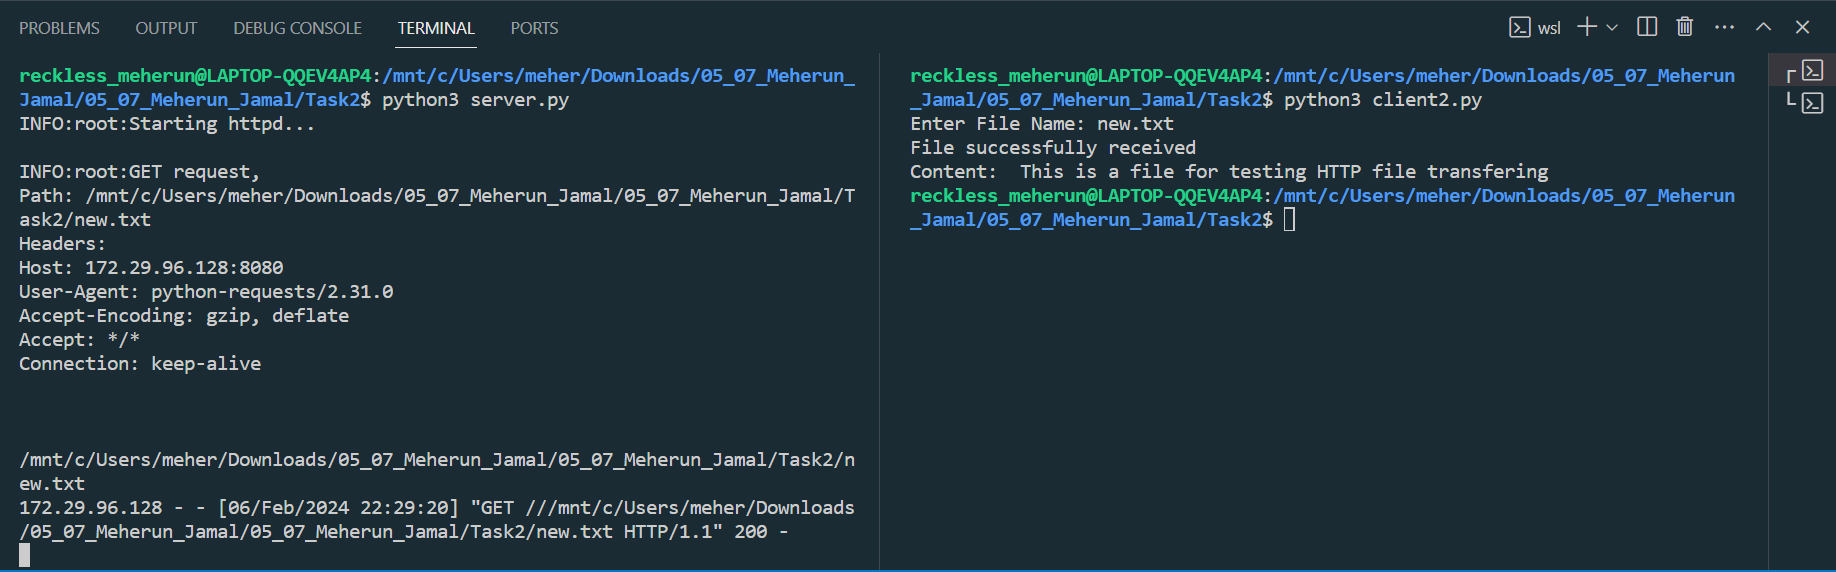
\includegraphics[scale=0.3]{Task2/T2_Get.png} 
    \caption{Output for Get}
    \label{fig: Output for Option 3}
\end{figure}

\begin{figure}[ht]
    \centering
    \caption{Output for Post}
    \label{fig: Output for Option 3}
\end{figure}

\newpage
\section{Experience}
\begin{enumerate}
\item We had to learn how to enable the server to handle multiple client at once.
\item We had to see some examples of how to use HttpServer package in Python
\end{enumerate}


\bibliographystyle{plain}
\bibliography{ref} % Assuming your BibTeX file is named "ref.bib"
\nocite{*}


\end{document}
